\documentclass{jhwhw}
\usepackage{amsmath}
\usepackage{amssymb}
\usepackage{tikz}
\usetikzlibrary{arrows}
%\usepackage[makeroom]{cancel}
%\usetikzlibrary{patterns}
\title{MATH 5510: Topology: HW 3}
\author{Markus Foote}

\newcommand{\R}{{\mathbb R}}
\newcommand{\C}{{\mathbb C}}
\newcommand{\Z}{{\mathbb Z}}
\newcommand{\Q}{{\mathbb Q}}
\newcommand{\N}{{\mathbb N}}
\newcommand{\T}{{\mathcal T}}

\begin{document}
\problem{}%1
 Consider two topologies on $\R$:  the Euclidean (or usual) topology $\T_E$, and the topology $\T_{CF}$ in which the \emph{closed} sets are $\R$ and all the finite subsets of $\R$.
 
 \begin{enumerate}
 	
 	\item Suppose $f:(\R,\T_E)\to (\R,\T_E)$ is continuous.  Prove that it is also continuous as a map $(\R,\T_E) \to (\R,\T_{CF})$.
 	
 	\item Give an example of  a continuous map $g:(\R,\T_E)\to (\R,\T_{CF})$ that is \emph{not} continuous as a map $(\R,\T_E)\to (\R,\T_E)$.
 	
 	\emph{Suggestion}:  Try strictly increasing piecewise linear maps.
 	
 	\item Find all continuous maps $f:(\R,\T_{CF})\to (\R,\T_E)$.
 \end{enumerate}
\solution{}
\part{}
Let $f: (\R,\T_E)\to(\R,\T_{CF})$. $f$ is continuous iff $\forall U \subset \R$ when $U$ closed in $\T_{CF} \implies f^{-1}(U)$ is closed in $\T_E$.
Let \begin{equation}U = \bigcup\limits_{i=1}^{N} x_i \end{equation} be a closed set in the topology $\T_{CF}$, then this set is also closed in $\T_E$ because a single point $x_i$ is closed and the closed sets are closed under finite union. The mapping $f:(\R,\T_E)\to(\R,\T_E)$ is continuous $\implies f^{-1}(U)$ is closed, thus $f$ is continuous. 

\part{}
A continuous map $g:(\R,\T_E)\to (\R,\T_{CF})$ that is \emph{not} continuous as $(\R,\T_E)\to (\R,\T_E)$ is \begin{equation}g(x) = \begin{cases} x & x\le 0 \\ x+1 & x >0 \end{cases}\end{equation} 
This map is continuous $\T_E \to \T_{CF}$ as the preimage of any finite set of points (which is closed in $\T_{CF}$) is closed in $\T_E$:
\begin{gather}
\text{Let } U= \bigcup\limits_{i=1}^{N} x_i\\
f^{-1}(U) = \left\{ \bigcup x_i \;\forall x_i \le 0 \right\} \cup \left\{\bigcup x_i+1 \; \forall x_i > 0\right\}
\end{gather}
where $x_i\in\R$, thus the preimage in $\T_E$ is a finite union of closed sets, which is also closed.

$g:(\R,\T_E)\to (\R,\T_E)$ is \emph{not} continuous because the preimage of a $\T_E$-closed set is not $\T_E$-closed:
\begin{gather}
\text{Let } U= \left[\frac{1}{2},\frac{3}{2}\right]\\
f^{-1}(U) = \left(0,\frac{1}{2}\right]
\end{gather}
This preimage is not $\T_E$-closed, so the map is not continuous, because a map is continuous iff the preimage of every closed set is closed.

These diagrams illustrate these cases:
\begin{center}
	\begin{tabular}{ccc}
		$g:(\R,\T_E)\to (\R,\T_{CF})$ cont.&\hspace{1cm}&$g:(\R,\T_E)\to (\R,\T_E)$ \emph{not} cont.\\
		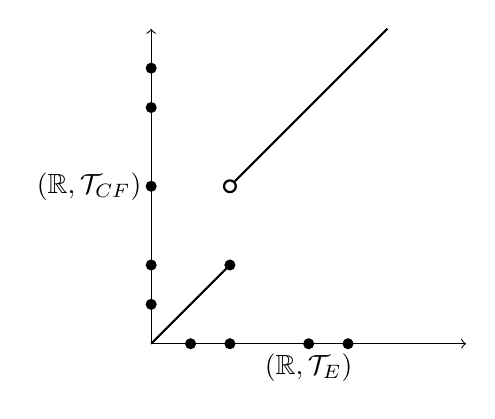
\begin{tikzpicture}
		%\draw [help lines] (0,0) grid (4,4);
		\draw [->](0,0) -- (0,4) node[midway,left] {$(\R,\T_{CF})$};
		\draw [->](0,0) -- (4,0) node[midway,below] {$(\R,\T_E)$};
		\draw [thick] (0,0) -- (1,1);
		\node [draw,circle,thick,inner sep=1.5pt] (c) at (1,2) {};
		\draw [thick] (c) -- (3,4);
		\fill (1,1) circle[radius=2pt];
		%draw the set in Y and its preimage
		\foreach \a in {0.5, 1,2, 3, 3.5}
			\fill (0,\a) circle[radius=2pt];
		\foreach \a in {0.5,1,2,2.5}
			\fill (\a,0) circle[radius=2pt];
		\end{tikzpicture}&&
		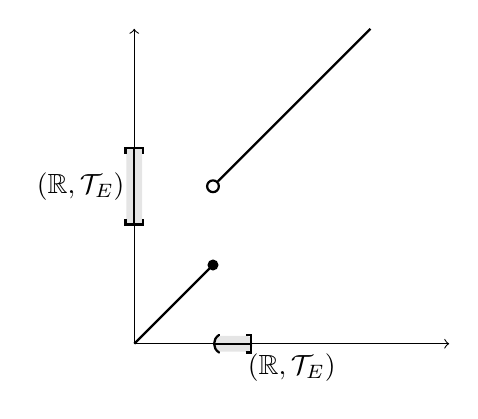
\begin{tikzpicture}
		%\draw [help lines] (0,0) grid (4,4);
		\draw [->](0,0) -- (0,4) node[midway,left] {$(\R,\T_{E})$};
		\draw [->](0,0) -- (4,0) node[midway,below] {$(\R,\T_E)$};
		\draw [thick] (0,0) -- (1,1);
		\node [draw,circle,thick,inner sep=1.5pt] (c) at (1,2) {};
		\draw [thick] (c) -- (3,4);
		\fill (1,1) circle[radius=2pt];
		%draw the set in Y and preimage
		\draw [(-, thick] (1,0) -- (1.5,0);
		\draw [[-, thick] (1.5,0) -- (1,0);
		\fill[opacity = 0.1,rounded corners=2pt] (1,-0.1) -- (1.5, -0.1) -- (1.5, 0.1) -- (1,0.1) -- cycle;
		\draw [[-, thick] (0,1.5) -- (0,2.5);
		\draw [[-, thick] (0,2.5) -- (0,1.5);
		\fill[opacity = 0.1,rounded corners=0.02pt] (-0.1,1.5) -- (-0.1, 2.5) -- (0.1, 2.5) -- (0.1,1.5) -- cycle;
		\end{tikzpicture}
	\end{tabular}
\end{center}
Note that for this $g$, $g^{-1}\big((1,2]\big)=\emptyset$, which is still closed.
\part{}


\problem{} %2
\begin{enumerate}
	\item Let $(X,\T_X)$ and $(Y,\T_Y)$ be topological spaces let $f,g:(X,\T_X)\to(Y,\T_Y)$ be continuous maps, and suppose that $(Y,\T_Y)$ is Hausdorff.   Prove that
	$$
	E(f,g) = \{x\in X \  | \  f(x) = g(x) \}
	$$
	is \emph{closed} in $(X,\T_X)$.
	\item Give an example of two continuous maps $f,g$ with $E(f,g)$ not closed.  (If possible, try to find an example with $(X,\T_X)$ 
	Hausdorff.)
\end{enumerate}

\solution{}

\part{}
Suppose $f(x) \neq g(x)$, because $Y$ is Hausdorff $\exists\: U = \text{nbd } \text{of } f(x),\; V=\text{nbd } \text{of } g(x)$ where $U\cap V=\emptyset$. The preimages of these open sets remain open as $f,g$ continuous, and since they both contain $x$: $f^{-1}(U),\:g^{-1}(V)\subset X$ are open nbds of $x$. Let $W=f^{-1}(U)\cap g^{-1}(V) \implies x\in W$. $W$ is still open as $\T_X$ is closed under finite intersection. These $x$ are such that $f(x)\neq g(x)$, so they are in the complement of $E$: $x\in W\subset E^{\mathsf{c}} \implies E^{\mathsf{c}} \text{ open } \implies E \text{ closed}$. 


\part{}



\problem{}%3
Let $(X,d)$ be a metric space, let $x\in X$ and let $A\subset X$ be non-empty.  Define the \emph{distance between $x$ and $A$}, denoted $d(x,A)$, by
$$
d(x,A) = \inf \{d(x,y)\  | \  y\in A\}.
$$
\begin{enumerate}
	\item Prove that $d(x,A)$ is a continuous function of $x$. 
	
	\emph{Suggestion}:  Prove more: it is a Lipschitz function, with Lipschitz constant $1$.
	
	\item Prove that $d(x,A) = 0\  \Longleftrightarrow \  x\in\overline{A}$.
	
	\item Prove that, if $A$ is closed, then there exists a continuous function $f:X\to\R$ so that $ A = \{x\in X | f(x) = 0\}$.
	
	
	
	\item Suppose $A,B\subset X$ are \emph{closed} sets, non-empty, and \emph{disjoint}: $A\cap B = \emptyset$. Prove that there exists a contiuous function $g:X\to [0,1]$ such that 
	$$
	g(x) = 0 \Longleftrightarrow x\in A \hbox{ and } g(x) = 1 \Longleftrightarrow x\in B.
	$$
	
	\emph{Suggestion}: Experiment with  functions with $d(x,A) + d(x,B)$ as denominator.
	
	\item Prove that if $A$ and $B$ are disjoint, non-empty, closed sets as above, there exist open sets $U,V\subset X$ so that $A\subset U, B\subset V$ and $U\cap V = \emptyset$.
\end{enumerate}

\solution{}
\part{}


\end{document}